\documentclass{beamer}
\mode<presentation>{
\usetheme{Warsaw}
\usecolortheme{sidebartab}
}
\usepackage{graphicx}
\usepackage{booktabs}
\usepackage{graphicx} 
\usepackage{booktabs} 
\usepackage[utf8x]{inputenc} 
\usepackage[T1]{fontenc}
\usepackage{geometry}     
\usepackage[francais]{babel} 
\usepackage{eurosym}
\usepackage{verbatim}
\usepackage{ragged2e}

\justifying
%%%%%%%%%%%%%%%%%%%%%%%%%%%%%%%%%%%%%%%%%%%%%%%%%%%%%%%%%%%%%%%%
%% ccBeamer 0.1, 2007-07-02                                   %%
%% Written by Sebastian Pipping <webmaster@hartwork.org>      %%
%% ---------------------------------------------------------- %%
%% Licensed under Creative Commons Attribution-ShareAlike 3.0 %%
%% http://creativecommons.org/licenses/by-sa/3.0/             %%
%%%%%%%%%%%%%%%%%%%%%%%%%%%%%%%%%%%%%%%%%%%%%%%%%%%%%%%%%%%%%%%%


%% Images
\newcommand{\CcImageBy}[1]{%
	\includegraphics[scale=#1]{creative_commons/cc_by_30.pdf}%
}
\newcommand{\CcImageCc}[1]{%
	\includegraphics[scale=#1]{creative_commons/cc_cc_30.pdf}%
}
\newcommand{\CcImageDevNations}[1]{%
	\includegraphics[scale=#1]{creative_commons/cc_dev_nations_30.pdf}%
}
\newcommand{\CcImageNc}[1]{%
	\includegraphics[scale=#1]{creative_commons/cc_nc_30.pdf}%
}
\newcommand{\CcImageNd}[1]{%
	\includegraphics[scale=#1]{creative_commons/cc_nd_30.pdf}%
}
\newcommand{\CcImagePd}[1]{%
	\includegraphics[scale=#1]{creative_commons/cc_pd_30.pdf}%
}
\newcommand{\CcImageSa}[1]{%
	\includegraphics[scale=#1]{creative_commons/cc_sa_30.pdf}%
}
\newcommand{\CcImageSampling}[1]{%
	\includegraphics[scale=#1]{creative_commons/cc_sampling_30.pdf}%
}
\newcommand{\CcImageSamplingPlus}[1]{%
	\includegraphics[scale=#1]{creative_commons/cc_sampling_plus_30.pdf}%
}


%% Groups
\newcommand{\CcGroupBy}[1]{% zoom
	\CcImageBy{#1}%
}
\newcommand{\CcGroupByNc}[2]{% zoom, gap
	\CcImageBy{#1}\hspace*{#2}\CcImageNc{#1}%
}
\newcommand{\CcGroupByNcNd}[2]{% zoom, gap
	\CcImageBy{#1}\hspace*{#2}\CcImageNc{#1}\hspace*{#2}\CcImageNd{#1}%
}
\newcommand{\CcGroupByNcSa}[2]{% zoom, gap
	\CcImageBy{#1}\hspace*{#2}\CcImageNc{#1}\hspace*{#2}\CcImageSa{#1}%
}
\newcommand{\CcGroupByNd}[2]{% zoom, gap
	\CcImageBy{#1}\hspace*{#2}\CcImageNd{#1}%
}
\newcommand{\CcGroupBySa}[2]{% zoom, gap
	\CcImageBy{#1}\hspace*{#2}\CcImageSa{#1}%
}
\newcommand{\CcGroupDevNations}[1]{% zoom
	\CcImageDevNations{#1}%
}
\newcommand{\CcGroupNcSampling}[2]{% zoom, gap
	\CcImageNc{#1}\hspace*{#2}\CcImageSampling{#1}%
}
\newcommand{\CcGroupPd}[1]{% zoom
	\CcImagePd{#1}%
}
\newcommand{\CcGroupSampling}[1]{% zoom
	\CcImageSampling{#1}%
}
\newcommand{\CcGroupSamplingPlus}[1]{% zoom
	\CcImageSamplingPlus{#1}%
}


%% Text
\newcommand{\CcLongnameBy}{Attribution}
\newcommand{\CcLongnameByNc}{Attribution-NonCommercial}
\newcommand{\CcLongnameByNcNd}{Attribution-NoDerivs}
\newcommand{\CcLongnameByNcSa}{Attribution-NonCommercial-ShareAlike}
\newcommand{\CcLongnameByNd}{Attribution-NoDerivs}
\newcommand{\CcLongnameBySa}{Attribution-ShareAlike}

\newcommand{\CcNote}[1]{% longname
	This work is licensed under the \textit{Creative Commons #1 3.0 License}.%
}


\title[Anonymity and encryption]{How to take back you privacy?}
\author{Naam, Genma}
\institute[@Gconfs]{
EPITA / Gconfs\\
\textit{naam@riseup.net\\ genma@riseup.net}
}
\date{01/17/13}
\begin{document}
\begin{frame}
\titlepage
\end{frame}
\begin{frame}
\frametitle{Overview}
\tableofcontents
\end{frame}
\section{Intro}
\subsection{Why we do this talk?}
%---------------------------------------------------
\begin{frame}
\frametitle{Sensitive data}
\begin{block}{Definition}
\begin{itemize}
\item a set of values of qualitative or quantitative variables
\item individual pieces of information
\end{itemize}
\end{block}
Some of them are (important|critical)s, don't play with Mallory.
\end{frame}
%---------------------------------------------------
\begin{frame}
\frametitle{The right to stay anonymous}
The Convention for the Protection of Human Rights and Fundamental Freedoms states
that :
\begin{block}{Article 8 - Right to respect for private and family life}
\begin{itemize}
\item Everyone has the right to respect for his private and family life (...).
\item  There shall be no interference by a public authority with the exercise
of this right except such as is in accordance with the law and is necessary in
a democratic society \emph{in the interests of national security, public safety or
the economic well-being of the country, for the prevention of disorder or crime,
for the protection of health or morals, or for the protection of the rights and
freedoms of others}.
\end{itemize}
\end{block}
\end{frame}
%--------------------------------------------------
\begin{frame}
\frametitle{You will also see}
\begin{itemize}
\item Tons of softwares, distributions, techniques to defeat too inquisitive
people and censorship.
\item What's a Cryptoparty and what you could learn from it.
\end{itemize}
\end{frame}
%--------------------------------------------------

\subsection{The digital identity}
%--------------------------------------------------
\begin{frame}
\end{frame}
%--------------------------------------------------

\subsection{Questions?}
%--------------------------------------------------
\begin{frame}
\frametitle{Something unclear ?}
\begin{columns}[c]
\column{.5\textwidth}
\begin{figure}
<<<<<<< HEAD

\includegraphics[width=0.8\linewidth]{./materials/questions.jpg}
=======

\includegraphics[width=0.8\linewidth]{./materials/questions}
>>>>>>> 591fd2d838dd16d11e0d639efe7605b36be9b3b9
\end{figure}
\column{.5\textwidth}
Feel free to ask for questions now.
\end{columns}
\end{frame}
%--------------------------------------------------

\section{HOW TO: Encryption}
\subsection{WTF is encryption?}

%------------------------------------------------
\begin{frame}
\frametitle{Definition - cryptage, encrypt, encryption ?}

\begin{block}{Encryption}
\justifying{
Encryption is to encrypt a document / file using an encryption key.
The reverse operation is decryption.
}
\end{block}
\begin{block}{Cryptage}
\justifying{
Term « cryptage » is derived from the English encryption and does not exist in French.
Decryption is the fact of breaking the encryption when the private key is unknown.
}
\end{block}
\begin{block}{Cryptography}
\justifying{
Science is called Cryptography.
}
\end{block}
\end{frame}

%------------------------------------------------
\begin{frame}
\frametitle{Encryption, how does it work?}

\begin{block}{Symetric Encryption}
\justifying{
This involves encrypting a message with the same key that will be used for decryption process.
\\
Sample : Caesar code,  with an offset letter. A->C, B->D etc.
\\
Nous venons en paix ->  Pqwu xgpqpu gp rckz
\\
The reverse process is applied to get the message.
}
\end{block}

\begin{block}{What is an encryption key?}
\justifying{

A key is called so because it opens / closes the padlock that is the used encryption algorithm.
\begin {itemize}
\item Here, the algorithm is the offset.
\item The key is the number of offset of letter (here two letters).
\end{itemize}
}
\end{block}

\end{frame}

%------------------------------------------------
\begin{frame}
\frametitle{Asymetric Encryption 1/2}

\begin{block}{Public key - Private key}
\justifying{

Asymetric Encryption is based on the pair public key - private key.
\\$\Rightarrow$ What you need to know: 
\begin{itemize}
\item My private key is... private and my own.
\item My public key is shared with everyone.
\end{itemize}
}
\end{block}
	
\begin{block}{The encryption algorithm}
\justifying{
The encryption algorithm is more complexe than the fact of shifting letters ; it is based on mathematical concepts (first number ...)
}
\end{block}

\end{frame}

\begin{frame}
\frametitle{Asymetric Encryption 2/2}

\begin{block}{Encryption}
With the public key of my correspondent, I encrypt a file.
\justifying{
\\$\Rightarrow$ The file can only be decrypted by the person who possesses the private key corresponding to the public key that I used (and therefore my correspondent).
}
\end{block}

\begin{block}{Decryption}
With its private key, my correspondent decrypts the file.
\\
$\Rightarrow$ He can then read the message.
\end{block}

\begin{block}{Concret case}
Mail Encryption with PGP.
\end{block}
\end{frame}

%----------------------------------------------------------------------------------------
\begin{frame}
\frametitle{Bob send a message to Alice}
\begin{center}
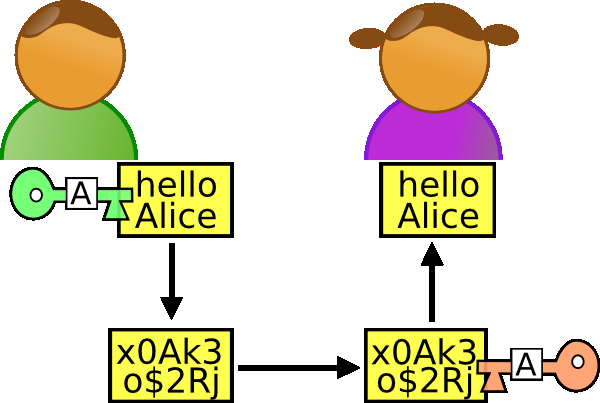
\includegraphics[scale=0.3] {./materials/Alice_et_bob} 
\end{center}
\end{frame}


%----------------------------------------------------------------------------------------
\begin{frame}
\Huge{\centerline{Why encryption?}}
\begin{center}
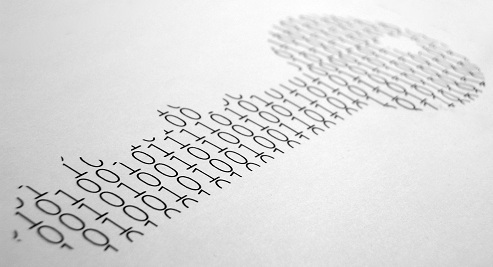
\includegraphics[scale=0.4] {./materials/cryptography.jpg} 
\end{center}
\end{frame}

%------------------------------------------------
\begin{frame}
\frametitle{Encrypt - The arguments against}

\justifying{
\begin{block}{Nobody does...}
FALSE. Without knowing it, you do it every day.
\\
Sample 1: "padlock" when connecting (https)
\\ Sample 2: Wifi key.
\end{block}

\begin{block}{Nothing to hide...}
FALSE. Who would accept the postman read his medical post ?
\end{block}

\begin{block}{Encryption, it's for the pedo-nazi...}
\justifying{
FALSE. For journalists / bloggers dissidents who are denouncing dictatorships...
}
\end{block}
}
\end{frame}

%------------------------------------------------
\begin{frame}
\frametitle{Encrypt - The arguments for}

\begin{block}{Encryption, it's not so complicated}
It is not more complicated than using a "software". You just have to understand the principle.
\end{block}

\begin{block}{Protection and security}
My personnal data are safe Cf. PRISM, NSA...
\end{block}

\begin{block}{Privacy}
Only the person for who the "message" is, is able to read it.
\end{block}

\end{frame}

%----------------------------------------------------------------------------------------
\begin{frame}
\frametitle{Edward Snowden}
\justifying{
Encryption works. Properly implemented strong crypto systems are one of the few things that you can rely on.
}
\begin{center}
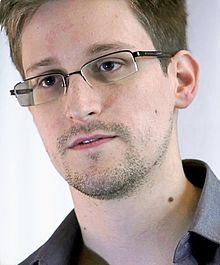
\includegraphics[scale=0.4] {./materials/snowden.jpg} 
\end{center}

\end{frame}


%------------------------------------------------
\begin{frame}
\frametitle{Encryption limit}
\begin{block}{Which is encrypted can be decrypted today tomorrow}
\justifying{
Tomorrow's computers will allow to decrypt the encrypted data today.
}
\end{block}

\begin{block}{It the private key is lost}
We no longer have access to data.
\end{block}

\begin{block}{Metadata, social graph}
\justifying{
\textbf{PGP does not protect against the analysis of metadata (servers transit, addresses, headers, subject).}
Do not forget to clean the meta-data files (EXIF tag photos, office documents with tracked changes).
DNS... Case of tracking Internet ...}
\end{block}

\end{frame}

%----------------------------------------------------------------------------------------
\begin{frame}
\frametitle{Law and encryption}
\justifying{
In France, the law therefore considers that the use of cryptology is free (LCEN Article 30-1) and there is therefore now no limit to the size of the encryption key that can be used .
\\~\\
In case of search, the refusal of submission of the encryption key may result in 3 years imprisonment and 45000\euro{}.
\\~\\
This penalty is increased if Encryption was used to commit a crime.
\\~\\
It is therefore recommended to give the decryption key, except in the case where the decrypted data would result in a judicial proceeding in which the final sentence would be greater than the interference with the judicial investigation.
}
\end{frame}



\subsection{What can I encrypt? How?}
%--------------------------------------------------
\begin{frame}
\end{frame}
%--------------------------------------------------

\subsection{Questions?}
%--------------------------------------------------
\begin{frame}
\frametitle{Something unclear ?}
\begin{columns}[c]
\column{.5\textwidth}
\begin{figure}
<<<<<<< HEAD

\includegraphics[width=0.8\linewidth]{./materials/questions.jpg}
=======

\includegraphics[width=0.8\linewidth]{./materials/questions}
>>>>>>> 591fd2d838dd16d11e0d639efe7605b36be9b3b9
\end{figure}
\column{.5\textwidth}
Feel free to ask for questions now.
\end{columns}
\end{frame}
%--------------------------------------------------

\section{HOW TO: Anonymity}
\subsection{Why does it matter?}
%--------------------------------------------------
\begin{frame}
\end{frame}
%--------------------------------------------------

\subsection{There is always a tool that fit your need}
%--------------------------------------------------
\begin{frame}
\end{frame}

\subsection{Questions?}
%--------------------------------------------------
\begin{frame}
\frametitle{Something unclear ?}
\begin{columns}[c]
\column{.5\textwidth}
\begin{figure}
<<<<<<< HEAD

\includegraphics[width=0.8\linewidth]{./materials/questions.jpg}
=======

\includegraphics[width=0.8\linewidth]{./materials/questions}
>>>>>>> 591fd2d838dd16d11e0d639efe7605b36be9b3b9
\end{figure}
\column{.5\textwidth}
Feel free to ask for questions now.
\end{columns}
\end{frame}

%--------------------------------------------------
\section{Conclusion}
\subsection{We're not in a XOXO word}
%--------------------------------------------------
\begin{frame}
\end{frame}
%--------------------------------------------------

\subsection{Cryptoparty}
%--------------------------------------------------
\begin{frame}
\end{frame}
%--------------------------------------------------

\subsection{Questions?}
%--------------------------------------------------
\begin{frame}
\frametitle{Something unclear ?}
\begin{columns}[c]
\column{.5\textwidth}
\begin{figure}
<<<<<<< HEAD

\includegraphics[width=0.8\linewidth]{./materials/questions.jpg}
=======

\includegraphics[width=0.8\linewidth]{./materials/questions}
>>>>>>> 591fd2d838dd16d11e0d639efe7605b36be9b3b9
\end{figure}
\column{.5\textwidth}
Feel free to ask for questions now.
\end{columns}
\end{frame}

%--------------------------------------------------
\begin{frame}
\frametitle{Rendez vous at the Cryptoparty}
\begin{figure}
<<<<<<< HEAD

\includegraphics[width=0.8\linewidth]{./materials/cryptoparty.jpg}
=======

\includegraphics[width=0.8\linewidth]{./materials/cryptoparty}
>>>>>>> 591fd2d838dd16d11e0d639efe7605b36be9b3b9
\end{figure}
\end{frame}
%--------------------------------------------------

\end{document}

